
\part*{Magnetismus}

Gesamtkraft auf eine Ladung:
\begin{verse}
$\vec{F}_{elmag}=Q(\vec{E}+\vec{v}\times\vec{B})$
\end{verse}

\section*{Lorentzkraft}
\begin{verse}
$\vec{F}_{L}=Q\vec{v}\times\vec{B}$ (Kreuzprodukt)

$\vec{v}=Geschwindigkeit$

$\vec{B}=Magnetfeld$
\end{verse}

\subsection*{Kreuzprodukt}
\begin{verse}
$\left(\begin{array}{c}
a_{1}\\
a_{2}\\
a_{3}
\end{array}\right)\times\left(\begin{array}{c}
b_{1}\\
b_{2}\\
b_{3}
\end{array}\right)=\left(\begin{array}{c}
a_{2}b_{3}-a_{3}b_{2}\\
a_{3}b_{1}-a_{1}b_{3}\\
a_{1}b_{2}-a_{2}b_{1}
\end{array}\right)$
\end{verse}

\section*{Zyklotronradius}
\begin{verse}
$|\vec{F}_{Zentrifugal}|=|\vec{F}_{Lorentz}|$

$\frac{mv^{2}}{r}=qvB$

$r=\frac{mv}{qB}$
\end{verse}
Zentrifugalkraft:
\begin{verse}
$\vec{a}(t)=\left(\begin{array}{c}
-r\omega^{2}cos(\omega t)\\
-r\omega^{2}sin(\omega t)
\end{array}\right)$

$\Rightarrow|\vec{a}(t)|=r\omega^{2}=\frac{|\vec{v}(t)|}{r}=\frac{v^{2}}{r}$
\end{verse}

\section*{Motoren und Generatoren}


\subsection*{Kraft auf Ströme}
\begin{itemize}
\item Ströme \textquotedbl{}bestehen\textquotedbl{} aus fliessenden Elektronen
\item Die \textquotedbl{}technische Stromrichtung\textquotedbl{} ist der
Flussrichtung der negativ geladenen Elektronen entgegengesetzt.
\item Steht ein stromdurchflossener Draht senkrecht zu einem Magnetfeld
wirkt eine Kraft auf den Draht.
\end{itemize}
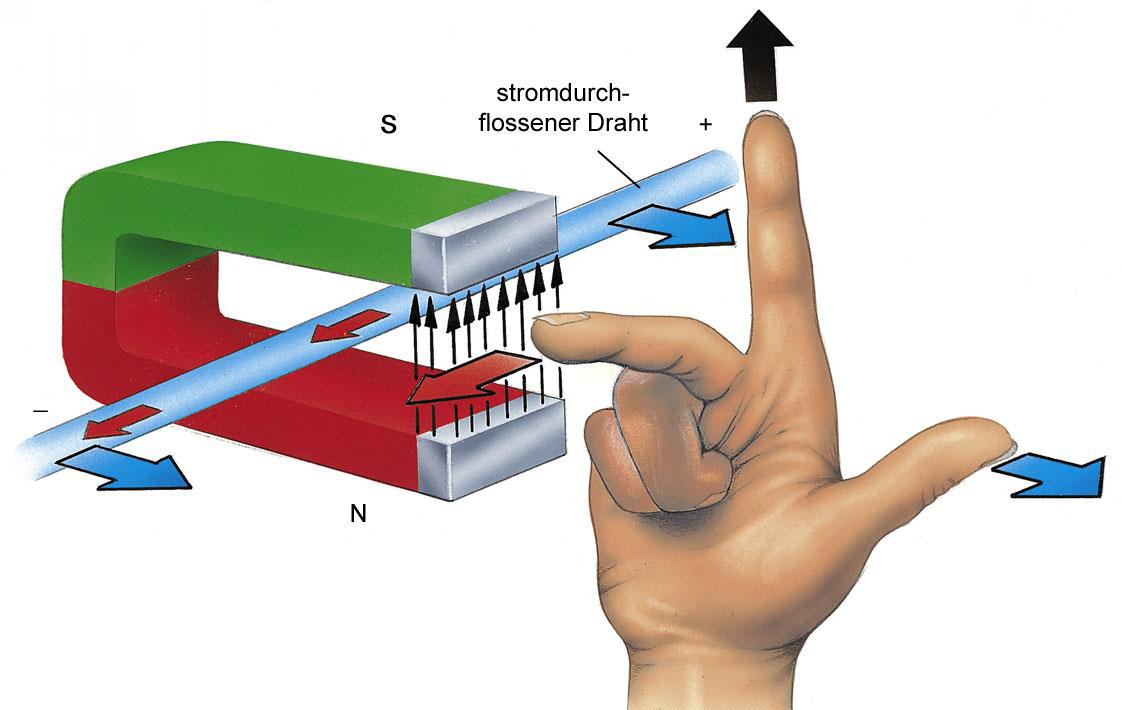
\includegraphics[scale=0.4]{Magnetismus/Lorentzkraft}
